\section{pgfplots}

Pgfplots can do basically any plot, more info \href{https://it.overleaf.com/learn/latex/Pgfplots_package}{here}

\subsubsection{Un grafico esponenziale}

\begin{verbatim}
\begin{tikzpicture}
    \begin{axis}
        \addplot[color=red]{exp(x)};
    \end{axis}
\end{tikzpicture}
%Here ends the furst plot
\hskip 5pt
%Here begins the 3d plot
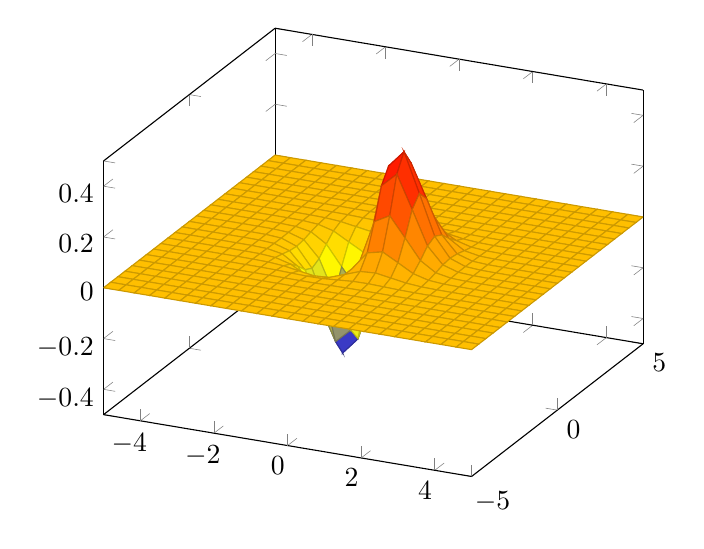
\begin{tikzpicture}
    \begin{axis}
        \addplot3[
                surf,
            ]
        {exp(-x^2-y^2)*x};
    \end{axis}
\end{tikzpicture}
\end{verbatim}

\begin{tikzpicture}
    \begin{axis}
        \addplot[color=red]{exp(x)};
    \end{axis}
\end{tikzpicture}
%Here ends the furst plot
\hskip 5pt
%Here begins the 3d plot
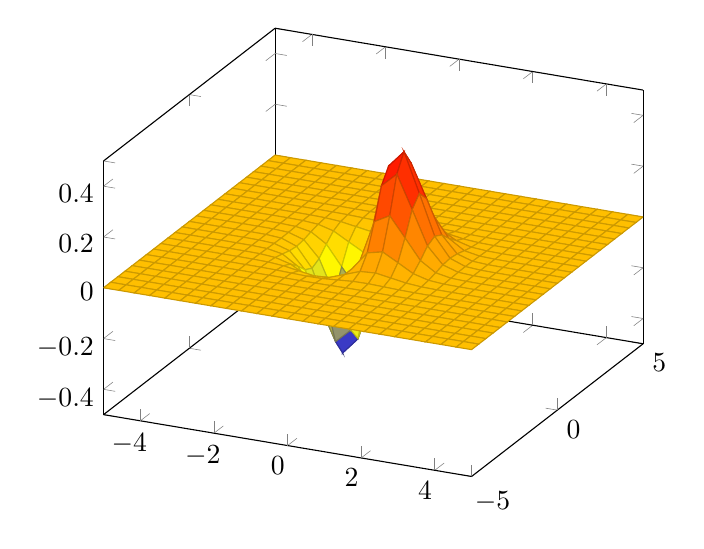
\begin{tikzpicture}
    \begin{axis}
        \addplot3[
                surf,
            ]
        {exp(-x^2-y^2)*x};
    \end{axis}
\end{tikzpicture}

\subsection{2D plots}

\begin{verbatim}
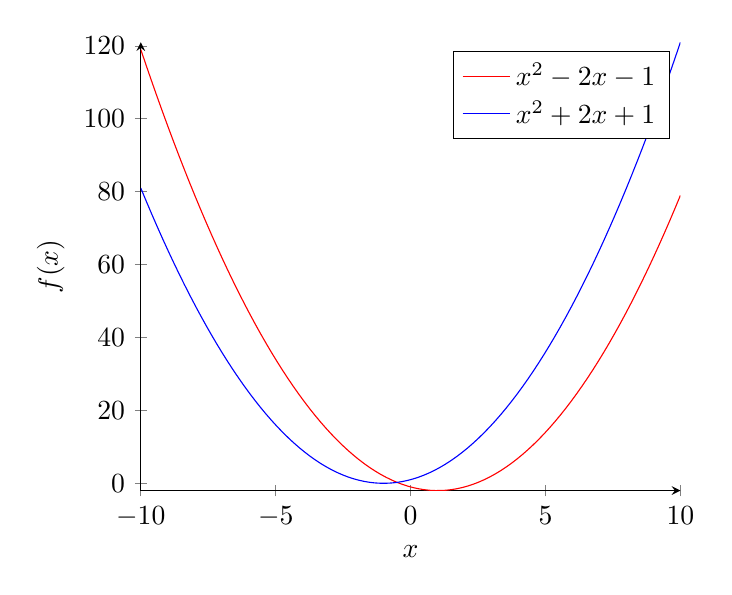
\begin{tikzpicture}
\begin{axis}[
    axis lines = left,
    xlabel = $x$,
    ylabel = {$f(x)$},
]
%Below the red parabola is defined
\addplot [
    domain=-10:10, 
    samples=100, 
    color=red,
]
{x^2 - 2*x - 1};
\addlegendentry{$x^2 - 2x - 1$}
%Here the blue parabloa is defined
\addplot [
    domain=-10:10, 
    samples=100, 
    color=blue,
    ]
    {x^2 + 2*x + 1};
\addlegendentry{$x^2 + 2x + 1$}
 
\end{axis}
\end{tikzpicture}
\end{verbatim}
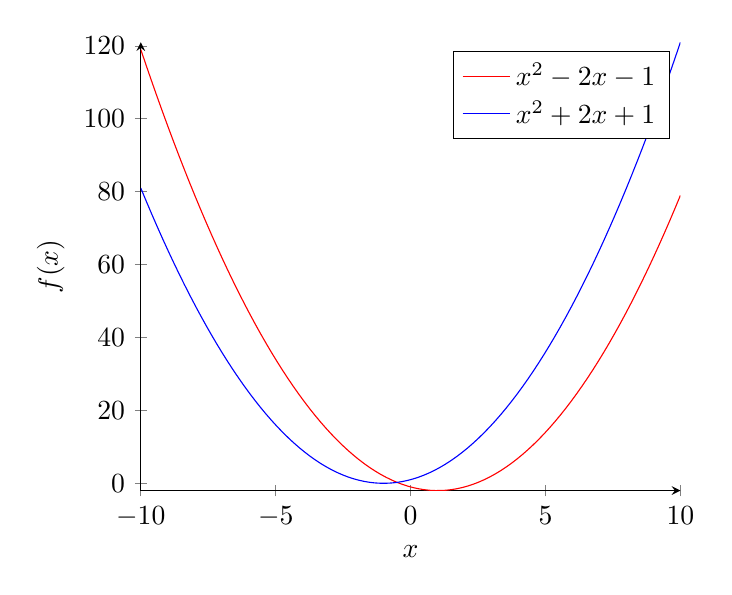
\begin{tikzpicture}
\begin{axis}[
    axis lines = left,
    xlabel = $x$,
    ylabel = {$f(x)$},
]
%Below the red parabola is defined
\addplot [
    domain=-10:10, 
    samples=100, 
    color=red,
]
{x^2 - 2*x - 1};
\addlegendentry{$x^2 - 2x - 1$}
%Here the blue parabloa is defined
\addplot [
    domain=-10:10, 
    samples=100, 
    color=blue,
    ]
    {x^2 + 2*x + 1};
\addlegendentry{$x^2 + 2x + 1$}
 
\end{axis}
\end{tikzpicture}




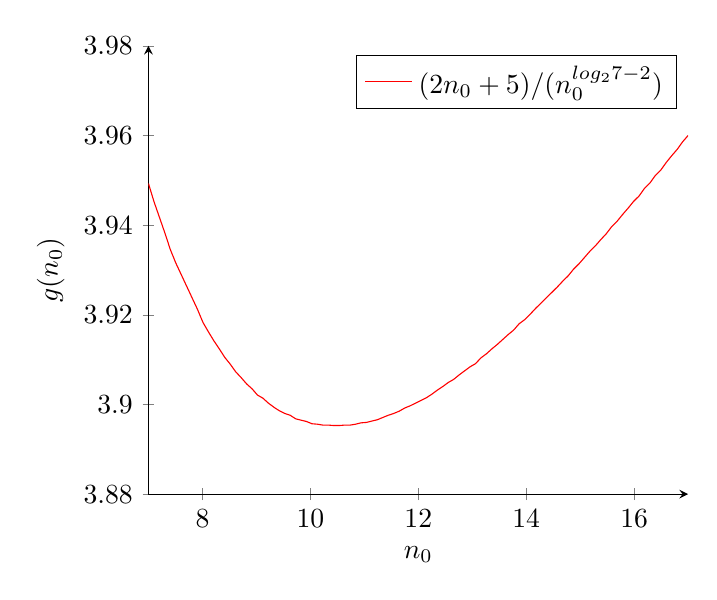
\begin{tikzpicture}
\begin{axis}[
    axis lines = left,
    xlabel = $n_0$,
    ylabel = {$g(n_0)$},
    ymin=3.88,
    ymax=3.98,
]
%Below the red parabola is defined
\addplot [
    % domain=0:20, 
    % domain=10:12, 
    domain=7:17, 
    samples=100, 
    color=red,
]
{(2*x+5)/(x^((2.807354922057604)-2) )};
% \addlegendentry{$\frac{2 n_0+5}{n_0^{log_2 7-2}}$}
\addlegendentry{$(2 n_0+5)/(n_0^{log_2 7-2})$}
%Here the blue parabloa is defined
% \addplot [
    % domain=-10:10, 
    % samples=100, 
    % color=blue,
    % ]
    % {x^2 + 2*x + 1};
% \addlegendentry{$x^2 + 2x + 1$}
 
\end{axis}
\end{tikzpicture}





